\documentclass[10pt]{article}



\usepackage{amsmath,amscd}
\usepackage{amssymb,array}
\usepackage{amsfonts,latexsym}
\usepackage{graphicx,subfig,wrapfig}
\usepackage{times}
\usepackage{psfrag,epsfig}
\usepackage{verbatim}
\usepackage{tabularx}
\usepackage[pagebackref=true,breaklinks=true,letterpaper=true,colorlinks,bookmarks=false]{hyperref}
\usepackage{cite}
\usepackage{algorithm}
\usepackage{multirow}
\usepackage{caption}
\usepackage{algorithmic}
\usepackage[amsmath,thmmarks]{ntheorem}
\usepackage{listings}
\usepackage{color}


\newtheorem{thm}{Theorem}
\newtheorem{mydef}{Definition}

\DeclareMathOperator*{\rank}{rank}
\DeclareMathOperator*{\trace}{trace}
\DeclareMathOperator*{\acos}{acos}
\DeclareMathOperator*{\argmax}{argmax}


\renewcommand{\algorithmicrequire}{ \textbf{Input:}}     
\renewcommand{\algorithmicensure}{ \textbf{Output:}}
\renewcommand{\mathbf}{\boldsymbol}
\newcommand{\mb}{\mathbf}
\newcommand{\matlab}[1]{\texttt{#1}}
\newcommand{\setname}[1]{\textsl{#1}}
\newcommand{\Ce}{\mathbb{C}}
\newcommand{\Ee}{\mathbb{E}}
\newcommand{\Ne}{\mathbb{N}}
\newcommand{\Se}{\mathbb{S}}
\newcommand{\norm}[2]{\left\| #1 \right\|_{#2}}

\newenvironment{mfunction}[1]{
	\noindent
	\tabularx{\linewidth}{>{\ttfamily}rX}
	\hline
	\multicolumn{2}{l}{\textbf{Function \matlab{#1}}}\\
	\hline
}{\\\endtabularx}

\newcommand{\parameters}{\multicolumn{2}{l}{\textbf{Parameters}}\\}

\newcommand{\fdescription}[1]{\multicolumn{2}{p{0.96\linewidth}}{
		
		\textbf{Description}
		
		#1}\\\hline}

\newcommand{\retvalues}{\multicolumn{2}{l}{\textbf{Returned values}}\\}
\def\0{\boldsymbol{0}}
\def\b{\boldsymbol{b}}
\def\bmu{\boldsymbol{\mu}}
\def\e{\boldsymbol{e}}
\def\u{\boldsymbol{u}}
\def\x{\boldsymbol{x}}
\def\v{\boldsymbol{v}}
\def\w{\boldsymbol{w}}
\def\N{\boldsymbol{N}}
\def\X{\boldsymbol{X}}
\def\Y{\boldsymbol{Y}}
\def\A{\boldsymbol{A}}
\def\B{\boldsymbol{B}}
\def\y{\boldsymbol{y}}
\def\cX{\mathcal{X}}
\def\transpose{\top} % Vector and Matrix Transpose

%\long\def\answer#1{{\bf ANSWER:} #1}
\long\def\answer#1{}
\newcommand{\myhat}{\widehat}
\long\def\comment#1{}
\newcommand{\eg}{{e.g.,~}}
\newcommand{\ea}{{et al.~}}
\newcommand{\ie}{{i.e.,~}}

\newcommand{\db}{{\boldsymbol{d}}}
\renewcommand{\Re}{{\mathbb{R}}}
\newcommand{\Pe}{{\mathbb{P}}}

\hyphenation{MATLAB}

\usepackage[margin=1in]{geometry}

\begin{document}
	
\title{Machine Learning, Spring 2023\\Homework 5}
\date{Due on 23:59 May 4, 2023} 
\maketitle

%%%%%--------------------

\section{Kernel function ($40$ points)}
Suppose we are given the following positively (``$+1$'') labeled data points $\mathbb{R}^2$:
$$
\begin{Bmatrix}
\begin{pmatrix}
1\\ 
1
\end{pmatrix} ,&
\begin{pmatrix}
1\\ 
-1
\end{pmatrix}  ,&
\begin{pmatrix}
-1\\ 
1
\end{pmatrix} ,&
\begin{pmatrix}
-1\\ 
-1
\end{pmatrix}
\end{Bmatrix},
$$
and the following negatively labeled (``$-1$'') data points in $\mathbb{R}^2$ (see Figure~\ref{fig:svm}):
$$
\begin{Bmatrix}
\begin{pmatrix}
2\\ 
2
\end{pmatrix} ,&
\begin{pmatrix}
2\\ 
-2
\end{pmatrix}  ,&
\begin{pmatrix}
-2\\ 
2
\end{pmatrix} ,&
\begin{pmatrix}
-2\\ 
-2
\end{pmatrix}
\end{Bmatrix}.
$$
\begin{figure}[h!]
	\centering
	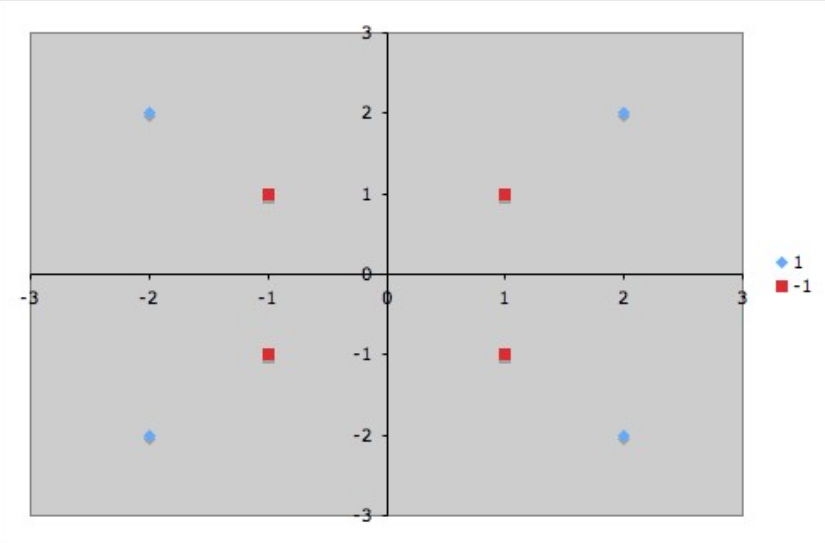
\includegraphics[width=3in]{svm.png}
	\caption{Blue diamonds are positive examples and red squares are negative examples.}
	\label{fig:svm}
\end{figure}	
\textbf{Question}: 
\begin{enumerate}
	\item Find a kernel function to map the data into a $\mathbb{R}^3$ feature space and make the new data linearly separable. (Show your kernel function please!) ($8$ points)
	\item Use SVM classifier to seperate the data. Show the SVM problem in your report. ($16$ points) Solve this SVM problem, write down the expression of the final separating hyperplane, and plot the data and the separating hyperplane in a figure. ($16$ points) (You can solve the SVM problem by apllying a convex problem solver.)
\end{enumerate}

\newpage

1. We can use the radial basis function (RBF) kernel to map the data into a higher dimensional space where they are linearly separable. The RBF kernel is defined as:

$$K(\mathbf{x}, \mathbf{y}) = \exp\left(-\frac{\|\mathbf{x}-\mathbf{y}\|^2}{2\sigma^2}\right)$$

where $\sigma$ is a hyperparameter that controls the spread of the kernel.

2. To solve the SVM problem, we first need to compute the kernel matrix $K$ where $K_{i,j} = K(\mathbf{x}_i, \mathbf{x}_j)$ for all $i,j$. We will use the RBF kernel with $\sigma=1$. Then, we can solve the dual problem:

$$\max_{\mathbf{\alpha}} \sum_{i=1}^{n}\alpha_i - \frac{1}{2}\sum_{i,j=1}^{n}\alpha_i\alpha_j y_i y_j K(\mathbf{x}_i,\mathbf{x}_j)$$

subject to $\alpha_i \geq 0$ for all $i$ and $\sum_{i=1}^{n}\alpha_iy_i = 0$. 

After solving the dual problem, we can compute the weight vector $\mathbf{w}$ and bias term $b$ for the optimal separating hyperplane as:

$$\mathbf{w} = \sum_{i=1}^{n}\alpha_i y_i \phi(\mathbf{x}_i)$$

$$b = y_k - \sum_{i=1}^{n}\alpha_i y_i K(\mathbf{x}_i,\mathbf{x}_k)$$

where $k$ is any index such that $0 < \alpha_k < C$. The separating hyperplane is given by the equation:

$$\mathbf{w}^T \phi(\mathbf{x}) + b = 0$$

To plot the data and the separating hyperplane in the 3D space induced by the RBF kernel, we can compute the feature vectors $\phi(\mathbf{x})$ for each data point, and then plot them in a 3D scatter plot. The separating hyperplane in the 3D space can be represented by a plane, and we can plot it by generating a grid of points in the plane and computing their corresponding class labels using the sign of $\mathbf{w}^T \phi(\mathbf{x}) + b$.

\begin{figure}[h!]
	\centering
	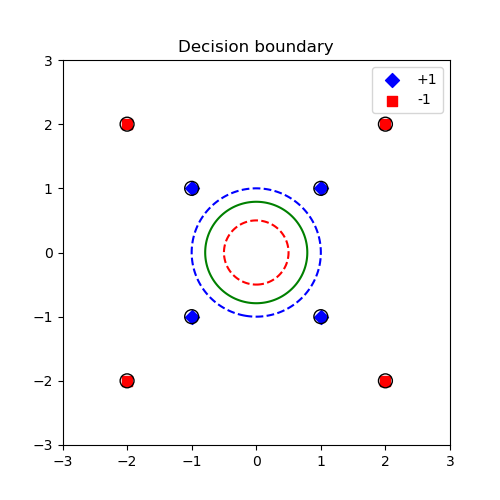
\includegraphics[width=3in]{1-1.png}
	\caption{Data points and the separating hyperplane in the $\mathbb{R}^3$ feature space induced.}
	\label{fig:svm_sol}
\end{figure}	
\newpage


\section{Cross Validation And L1 Regularization($60$ points)}
Given the training data set ``crime-train.txt''  and the test data set ``crime-test.txt'', you can read them in the files with in Python:
\begin{verbatim}
import pandas as pd
df_train = pd.read_table("crime-train.txt")
df_test = pd.read_table("crime-test.txt")
\end{verbatim}
This stores the data as Pandas DataFrame objects. DataFrames are similar to Numpy arrays but more flexible; unlike Numpy arrays, they store row and column indices along with the values of the data. Each column of a DataFrame can also, in principle, store data of a different type. For this assignment, however, all data are floats. Here are a few commands that will get you working with Pandas for this assignment:

\begin{verbatim}
df.head()                   # Print the first few lines of DataFrame df.
df.index                    # Get the row indices for df.
df.columns                  # Get the column indices.
df[``foo''']                # Return the column named ``foo'''.
df.drop(``foo'', axis = 1)  # Return all columns except ``foo''.
df.values                   # Return the values as a Numpy array.
df[``foo'''].values         # Grab column foo and convert to Numpy array.
df.iloc[:3,:3]              # Use numerical indices (like Numpy) to get 3 rows and cols.
\end{verbatim}

The data consist of local crime statistics for 1,994 US communities. The response $y$ is the crime rate. The name of the response variable is \texttt{ViolentCrimesPerPop}, and it is held in the first column of \texttt{df\_train} and \texttt{df\_test}. There are 95 features $x_i$. These features include possibly relevant variables such as the size of the police force or the percentage of children that graduate high school. The data have been split for you into a training and test set with 1,595 and 399 entries, respectively\footnote{The features have been standardized to have mean 0 and variance 1.}.

We'd like to use the training set to fit a model which can predict the crime rate in new communities, and evaluate model performance on the test set. As there are a considerable number of input variables, overfitting is a serious issue. In order to avoid this, implement the L1 regularization. 


The main goal of this homework is to give you some experience using L1 regularization as a method for variable selection and using 10-folder cross-validation as a technique to get an insight on how the model will generalize to an independent dataset.Your function should accept a scalar value of $\lambda$, a vector-valued response variable ($\mathbf{y}$), a matrix of input variables ($\mathbf{X}$), and an initial vector of weights ($\mathbf{w}_0$). It should output a vector of coefficient values ($\hat{\mathbf{w}}$).

Moreover, in order to solve the Lasso problem, we want you to implement the following algorithm. 

Consider the following generalized Lasso problem
\begin{equation} \label{glasso}
\begin{aligned}
\underset{\mb{x}} {\text{ min}} \  \frac{1}{2} \norm{\mb{A}\mb{x}-\mb{b}}{2}^2 + \lambda \norm{\mb{F}\mb{x}}{1}, 
\end{aligned}
\end{equation}
where $\mb{A}$ is the under-determined sensing matrix, $\mb{F}$ is the transformed matrix. In particular, it can be reduced to Lasso problem if $\mb{F} = \mb{I}$. The above problem is equivalent to the following formulation
\begin{equation} \label{glasso_adm}
\begin{aligned}
&\underset{\mb{x}, \mb{z}} {\text{ min}} \  \frac{1}{2} \norm{\mb{A}\mb{x}-\mb{b}}{2}^2 + \lambda \norm{\mb{z}}{1} \\
& \ \text{s.t.} \ \mb{F}\mb{x} = \mb{z},
\end{aligned}
\end{equation}
and one can employ augmented Lagrangian multiplier method to solve it. Specifically, the augmented Lagrangian is 
\begin{equation*}
\mathcal{L} = \frac{1}{2} \norm{\mb{A}\mb{x}-\mb{b}}{2}^2 + \lambda \norm{\mb{z}}{1} + <\mb{y}, \mb{F}\mb{x}- \mb{z}> + \frac{1}{2} \rho \norm{\mb{F}\mb{x} - \mb{z}}{2}^2,
\end{equation*}
which yields the ADMM algorithm, see Algorithm \ref{alg_glasso}. The soft-thresholding operator $\Se_{\frac{\lambda}{\rho}}$ is defined as 
\begin{equation}
\Se_{\frac{\lambda}{\rho}} (x_i) = \begin{cases}
x_i - \frac{\lambda}{\rho}, \ x_i \geq \frac{\lambda}{\rho} \\
0, \ |x_i| < \frac{\lambda}{\rho} \\
x_i + \frac{\lambda}{\rho}, \ x_i \leq -\frac{\lambda}{\rho}.
\end{cases}
\end{equation} 
\begin{algorithm}[h]
	\caption{ALM for generalized Lasso problem}
	\label{alg_glasso}
	\begin{algorithmic}[1] 
		\REQUIRE $\mb{A}, \mb{F}, \mb{b}, \lambda, \mu \ (\text{for augmented Lagrange multiplier})$
		\STATE Initialized $\rho, \mb{x}_0, \mb{z}_0,$ and $\mb{y}_0$, $k = 0$
		\WHILE {not converged}
		\STATE $\mb{x}^{(k+1)} = update \ \mb{x} ?$
		\STATE $\mb{z}^{(k+1)} = update \ \mb{z} ?$ (you may want to use $\Se_{\frac{\lambda}{\rho}}$ element-wise)
		\STATE $\mb{y}^{(k+1)} = \mb{y}^{(k)} + \rho (\mb{F} \mb{x}^{(k+1)} - \mb{z}^{(k+1)})$
		\STATE $\rho = \rho \mu$
		\STATE $k = k + 1$
		\ENDWHILE
		\ENSURE $\mb{x}^{*} = \mb{x}^{(k)}$
	\end{algorithmic}
\end{algorithm}




In your analysis, you need to finish:
\begin{enumerate}
	\item  Derive the steps of update x and z in Algorithm 1. (10 points)
	\item  A plot of $\log(\lambda)$ against the squared error in the 10-folder splited training data. (15 points)
	\item  A plot of $\log(\lambda)$ against the squared error in the test data. (10 points)
	\item  A plot of $\lambda$ against the number of small coefficients (you can set a threshold), and a brief commentary on the task of selecting $\lambda$. (15 points)
	\item  For the $\lambda$ that gave the best test set performance, which variable had the largest (most positive) coefficient? What about the most negative? Discuss briefly.  (10 points)
\end{enumerate}

\newpage
1. Derive the steps of update x and z in Algorithm 1. (10 points)

To update $\mathbf{x}$ and $\mathbf{z}$, we first compute the partial derivatives of the augmented Lagrangian $\mathcal{L}$ with respect to $\mathbf{x}$ and $\mathbf{z}$, and set them to zero.

For $\mathbf{x}$ update, differentiate $\mathcal{L}$ with respect to $\mathbf{x}$ and set it to zero:

$$\frac{\partial \mathcal{L}}{\partial \mathbf{x}} = \mathbf{A}^T(\mathbf{A}\mathbf{x}-\mathbf{b}) + \mathbf{F}^T(\mathbf{y} + \rho (\mathbf{F}\mathbf{x} - \mathbf{z})) = 0$$

Solve for $\mathbf{x}$:

$$\mathbf{x}^{(k+1)} = (\mathbf{A}^T\mathbf{A} + \rho \mathbf{F}^T\mathbf{F})^{-1}(\mathbf{A}^T\mathbf{b} + \rho \mathbf{F}^T(\mathbf{z}^{(k)} - \frac{1}{\rho}\mathbf{y}^{(k)}))$$

For $\mathbf{z}$ update, differentiate $\mathcal{L}$ with respect to $\mathbf{z}$ and set it to zero:

$$\frac{\partial \mathcal{L}}{\partial \mathbf{z}} = \lambda \frac{\mathbf{z}}{\lVert \mathbf{z} \rVert_1} - \mathbf{y} - \rho (\mathbf{F}\mathbf{x}^{(k+1)} - \mathbf{z}) = 0$$

Solve for $\mathbf{z}$:

$$\mathbf{z}^{(k+1)} = \Se_{\frac{\lambda}{\rho}}(\mathbf{F}\mathbf{x}^{(k+1)} + \frac{1}{\rho}\mathbf{y}^{(k)})$$

\begin{figure}[h!]
	\centering
	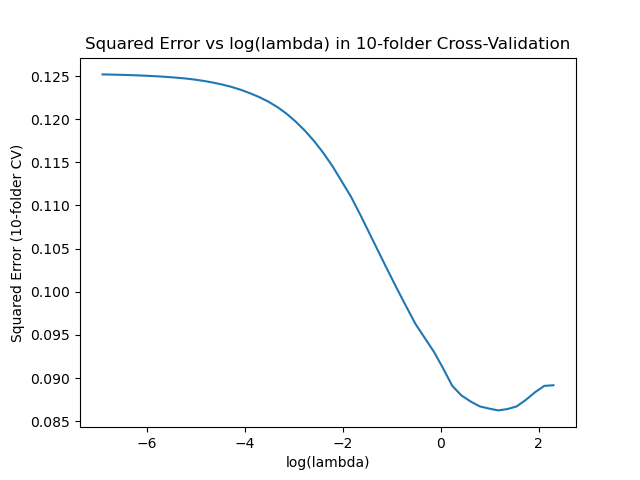
\includegraphics[width=3in]{2-2.png}
	\caption{A plot of $\log(\lambda)$ against the squared error in the 10-folder splited training data.}
	\label{fig:svm_sol}
\end{figure}	


\begin{figure}[h!]
	\centering
	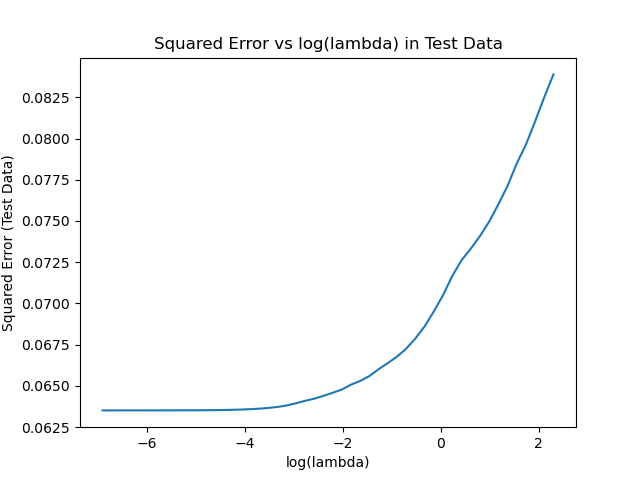
\includegraphics[width=3in]{2-3.png}
	\caption{A plot of $\log(\lambda)$ against the squared error in the test data.}
	\label{fig:svm_sol}
\end{figure}	


\begin{figure}[h!]
	\centering
	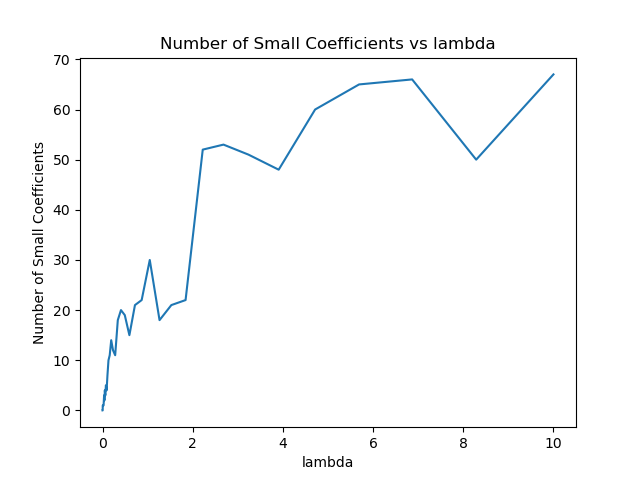
\includegraphics[width=3in]{2-4.png}
	\caption{A plot of $\lambda$ against the number of small coefficients (you can set a threshold), and a brief commentary on the task of selecting $\lambda$.}
	\label{fig:svm_sol}
\end{figure}	



\end{document} 